\chapter{Begriffsbestimmungen}
\subsubsection{\atmansf} \label{beg:atmans}
    
    Air Traffic Managament/Air Navigation Services (\atmans) -- definiert in \vo{VO}{EU}{2018/1139} Art. 3 Abs. 5 -- bezeichnet alle Aufgabenbereiche aus dem \acf{ATM}, der \acf{ANS} sowie der \acf{FPD} (siehe Abbildung \ref{fig:atmans}).
    Die jeweiligen Dienste und Funktionen dieser Bereiche werden im Zuge der \ac{SES} Rahmenverordnung (siehe \ref{er_549}) definiert.
    
    \begin{figure}[h!]
        \centering
        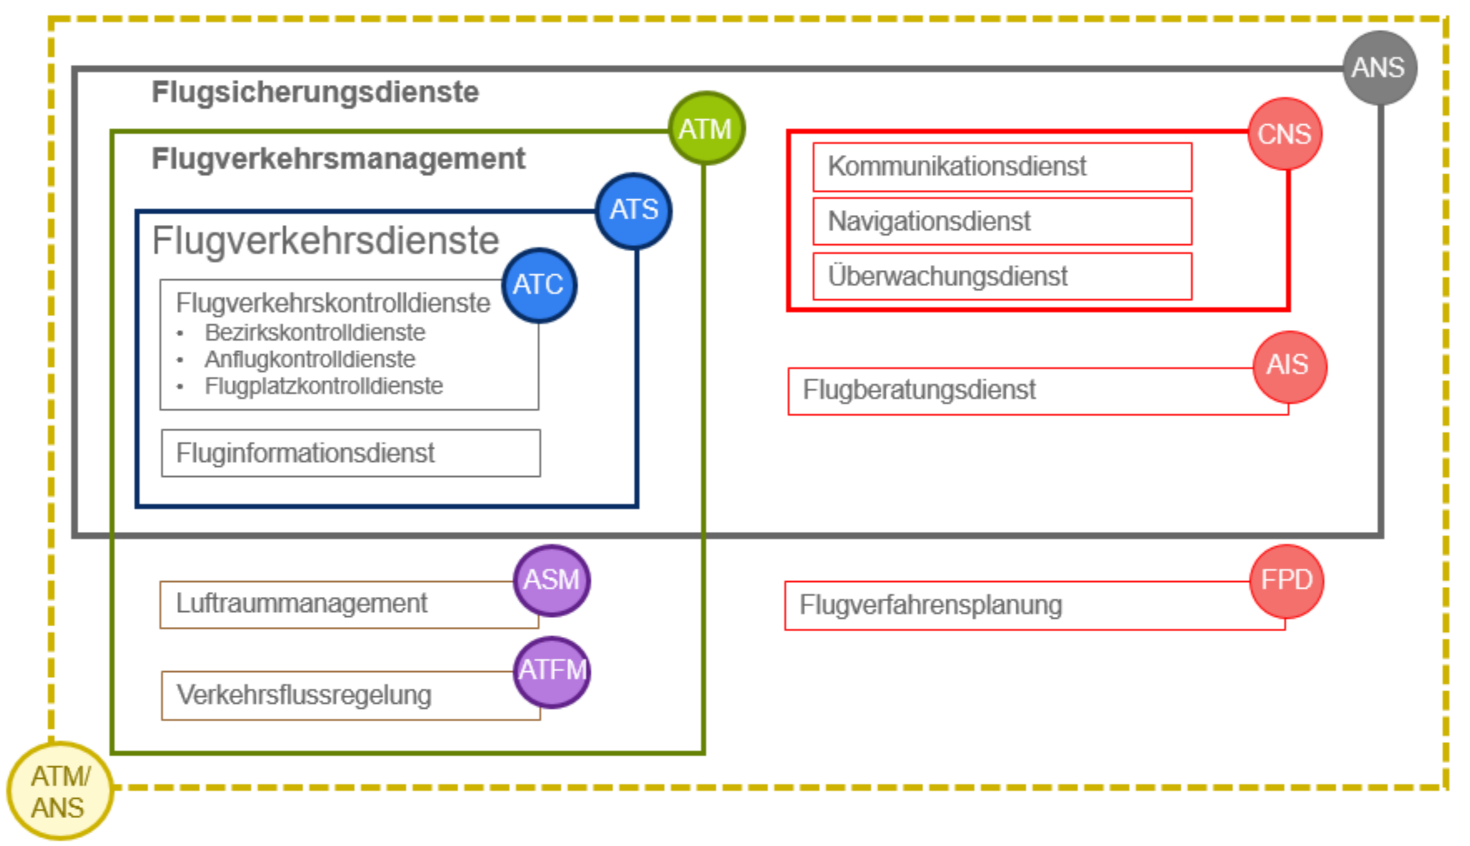
\includegraphics[width=\linewidth]{gfx/atmans.png}
        \caption{\atmansf-Definition \cite{ba_technik}}
        \label{fig:atmans}
    \end{figure}
    \acused{ATM}
    \acused{ATS}
    \acused{ATC}
    \acused{ASM}
    \acused{ATFM}
    \acused{AIS}
    \acused{FDP}
    \acused{ATM}
    \acused{ANS}

    \noindent
    Durch den rechtlichen Rahmen der \vo{DVO}{EU}{2017/373} und der national verantwortlichen Behörde werden lokale \acf{ANSP} für die oben aufgelisteten Aufgabenbereiche zertifiziert.
    Die \ac{DFS} verfügt hierbei über die Zertifizierung für die Erbringung aller in Abbildung \ref{fig:atmans} genannten \atmans-Dienste im deutschen Zuständigkeitsbereich. \cite[vgl.][17]{ba_technik}
    
    % \medskip
    % \begin{itemize}
    %     \item \acf{ATS}, bestehend aus
    %     \begin{itemize}
    %         \item \acf{ATC},
    %         \item Flugalarmdienst,
    %         \item Fluginformationsdienst;
    %     \end{itemize}
    %     \item Kommunikationsdienst (C);
    %     \item Navigationsdienst (N);
    %     \item Überwachungsdienst (S);
    %     \item \acf{AIS};
    %     \item \acf{ATFM};
    %     \item \acf{ASM};
    %     \item \acf{FPD}
    % \end{itemize}

\subsubsection{\atmansf-Equipment}
    
    \textit{\atmans-Equipment} (oder auch \textit{\atmans-Ausrüstung}), definiert in der \acf{DVO} \acs{EU} 2023/1769 Art. 2 Abs. 1, bestimmt sowohl \textit{Systeme} als auch \textit{Komponenten}, welche zur Erbringung der Dienste im \textit{funktionalen System} beitragen.
    \cite[Art.2 Abs.1]{2023R1769}

\subsubsection{\atmansf-Komponenten}

    \textit{\atmans-Komponenten} (im Folgenden auch \textit{Komponenten}) definieren nach \vo{VO}{EU}{2023/1769} Art. 2 Abs. 6  alle bezeichnet sowohl materielle Objekte wie Geräte als auch immaterielle Objekte wie Software, von denen die Interoperabilität des \ac{EATMN} abhängt.
    \cite[Art.2 Abs.6]{2023R1769}

\subsubsection{\atmansf-Systeme}

    \textit{\atmans-Systeme} (im Folgenden auch \textit{Systeme}) definieren nach der gleichen Verordnung die Zusammenfassung u.a. bodengestützter \textit{Komponenten}, welche eine Unterstützung für Flugsicherungsdienste aller Flugphasen bieten. 
    \cite[Art.2 Abs.7]{2023R1769}

\subsubsection{Compliance-Erklärung}

    Die \textit{Compliance-Erklärung} (oder auch \textit{Erklärung}) bezeichnet jede schriftliche Aussage eines \atmans-Anbieters, welche bestätigt, dass alle anwendbaren Anforderungen aus den einschlägigen Bestimmungen einer \atmans-Ausrüstung, erfüllt sind. 
    \cite[Art.2 Abs.10]{2018R1139}

\subsubsection{Funktionales System}

    Ein \textit{Funktionales System} (engl. \textit{functional system}) beschreibt nach der \vo{DVO}{EU}{2017/373} ,,eine Kombination von Verfahren, Personal und \textit{Ausrüstung}, einschließlich Hardware und Software, zur Erfüllung einer Funktion im Bereich \atmans{} und sonstiger Funktionen des Flugverkehrsmanagementnetzes``\cite[Anh.I Abs.56]{2017R0373}.
    Die \ac{DFS} wird im Rahmen der oben definierten Aufgabenbereiche auch als Gesamt-Funktionales System (auch \textit{Gesamtsystem Flugsicherung}) qualifiziert.
    \cite[17]{ba_technik}

\subsubsection{Impact Analyse}

    Eine \textit{Impact Analyse} -- dessen genaue Definition aus dem Kapitel \ref{model_ia} hervorgeht -- beschreibt das abstrakte Konzept, vernetzte Entitäten im Hinblick auf eine primäre Änderung zu analysieren.
    Die \textit{Impact Analyse} zieht in Betracht, welche Entitäten im System vorliegen und wie diese miteinander verknüpft sind. 
    Folglich kann ermittelt werden, wie sich eine primäre Änderung auf die weiteren Entitäten auswirkt.